\section{\name: IO \& Activity Privacy}
\label{sec:IOPrivacy}

Now we extend the capability of \name to provide privacy to generic IO devices.

\subsection{Input privacy}
\label{sec:systemDesign:inputPrivacy}

\name provides input privacy from the malicious host. The input privacy feature keeps the malicious host from knowing the sensitive input from the user to the remote server. The outline of the protocol is illustrated in Figure~\ref{fig:inputPrivacy}. The flow of the protocol is as the following:

\begin{enumerate}
  \item[\one] User input from the keyboard to the \device.
  \item[\two] The \device encrypts the data and sends to the host.
  \item[\three] The host renders the frame and send it to the \device.
  \item[\four] The \device overlays the plain text information on the frame and sends it to the display device.
\end{enumerate}


\begin{figure}[h]
\centering
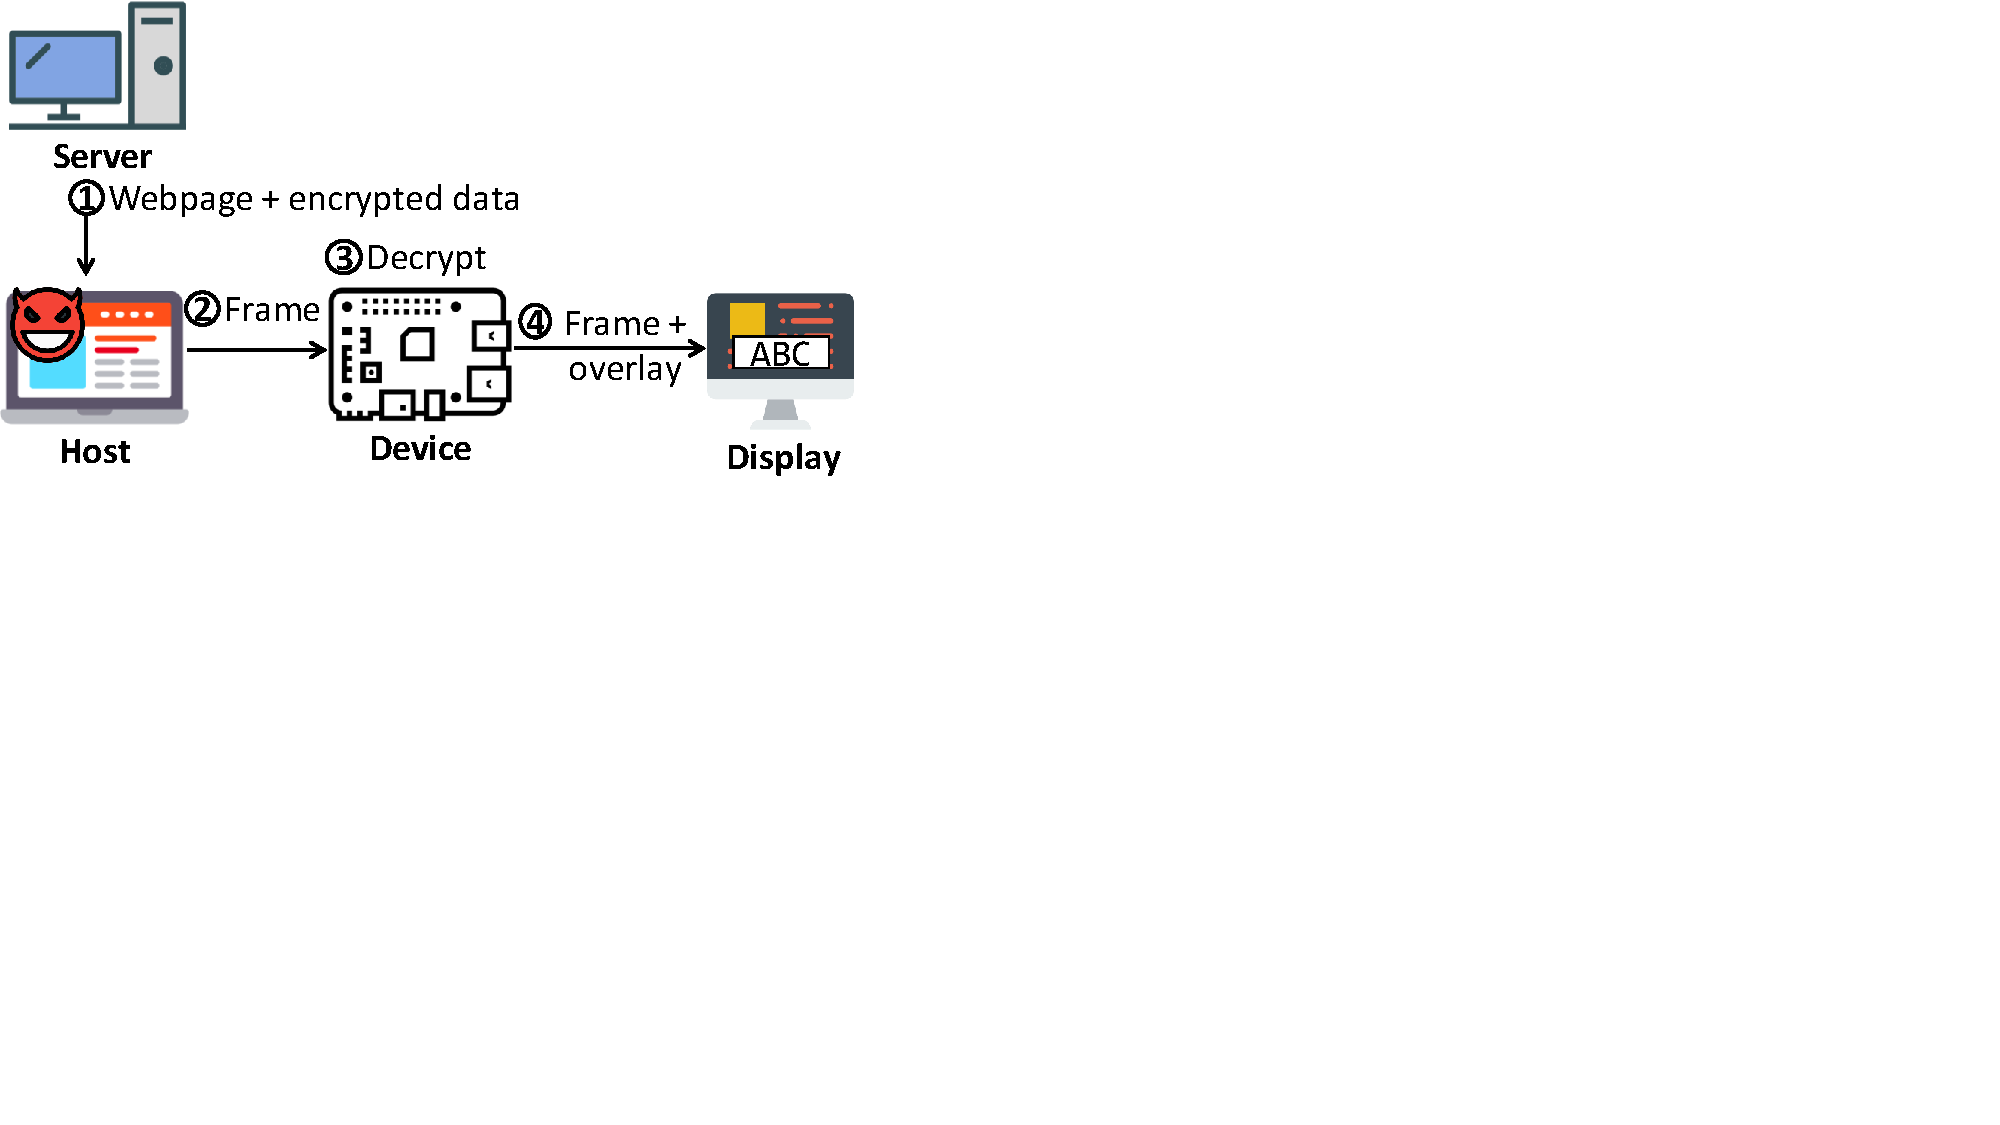
\includegraphics[trim={0 11cm 19cm 0}, clip, width=\linewidth]{outputPrivacy.pdf}
\caption{Output privacy}
\label{fig:outputPrivacy}
\centering
\end{figure}

\iffalse
\lstset{language=HTML, frame=tb, caption=\textbf{Partially encrypted HTML page.} , label = snippet:encryptedHTML, firstnumber =1}
\begin{figure}[t]
\small
\begin{lstlisting}[mathescape=true]
<!DOCTYPE html>
<html> <body>
<form action="/some_action">
  First name:<br>
  <input type="text" name="First name">
  <br> Last name:<br>
  <input type="text" name="name">
  <encrypted>
  [encrypted data]
  </encrypted>
  <input type="submit" value="Submit">
</form> </body> </html>
\end{lstlisting} 
\end{figure}


\lstset{language=HTML, frame=tb, caption=\textbf{Equivalent decrypted HTML page of Specification~\ref{snippet:encryptedHTML}.} , label = snippet:decryptedHTML, firstnumber =1}
\begin{figure}[t]
\small
\begin{lstlisting}[mathescape=true]
<!DOCTYPE html>
<html> <body>
<form action="/some_action">
  First name:<br>
  <input type="text" name="First name">
  <br> Last name:<br>
  <input type="text" name="name">
  <input type="radio" name="candidate1"> Candidate 1
  <input type="radio" name="candidate2"> Candidate 2
  <input type="submit" value="Submit">
</form> </body> </html>
\end{lstlisting} 
\end{figure}
\fi



\begin{figure}[h]
\centering
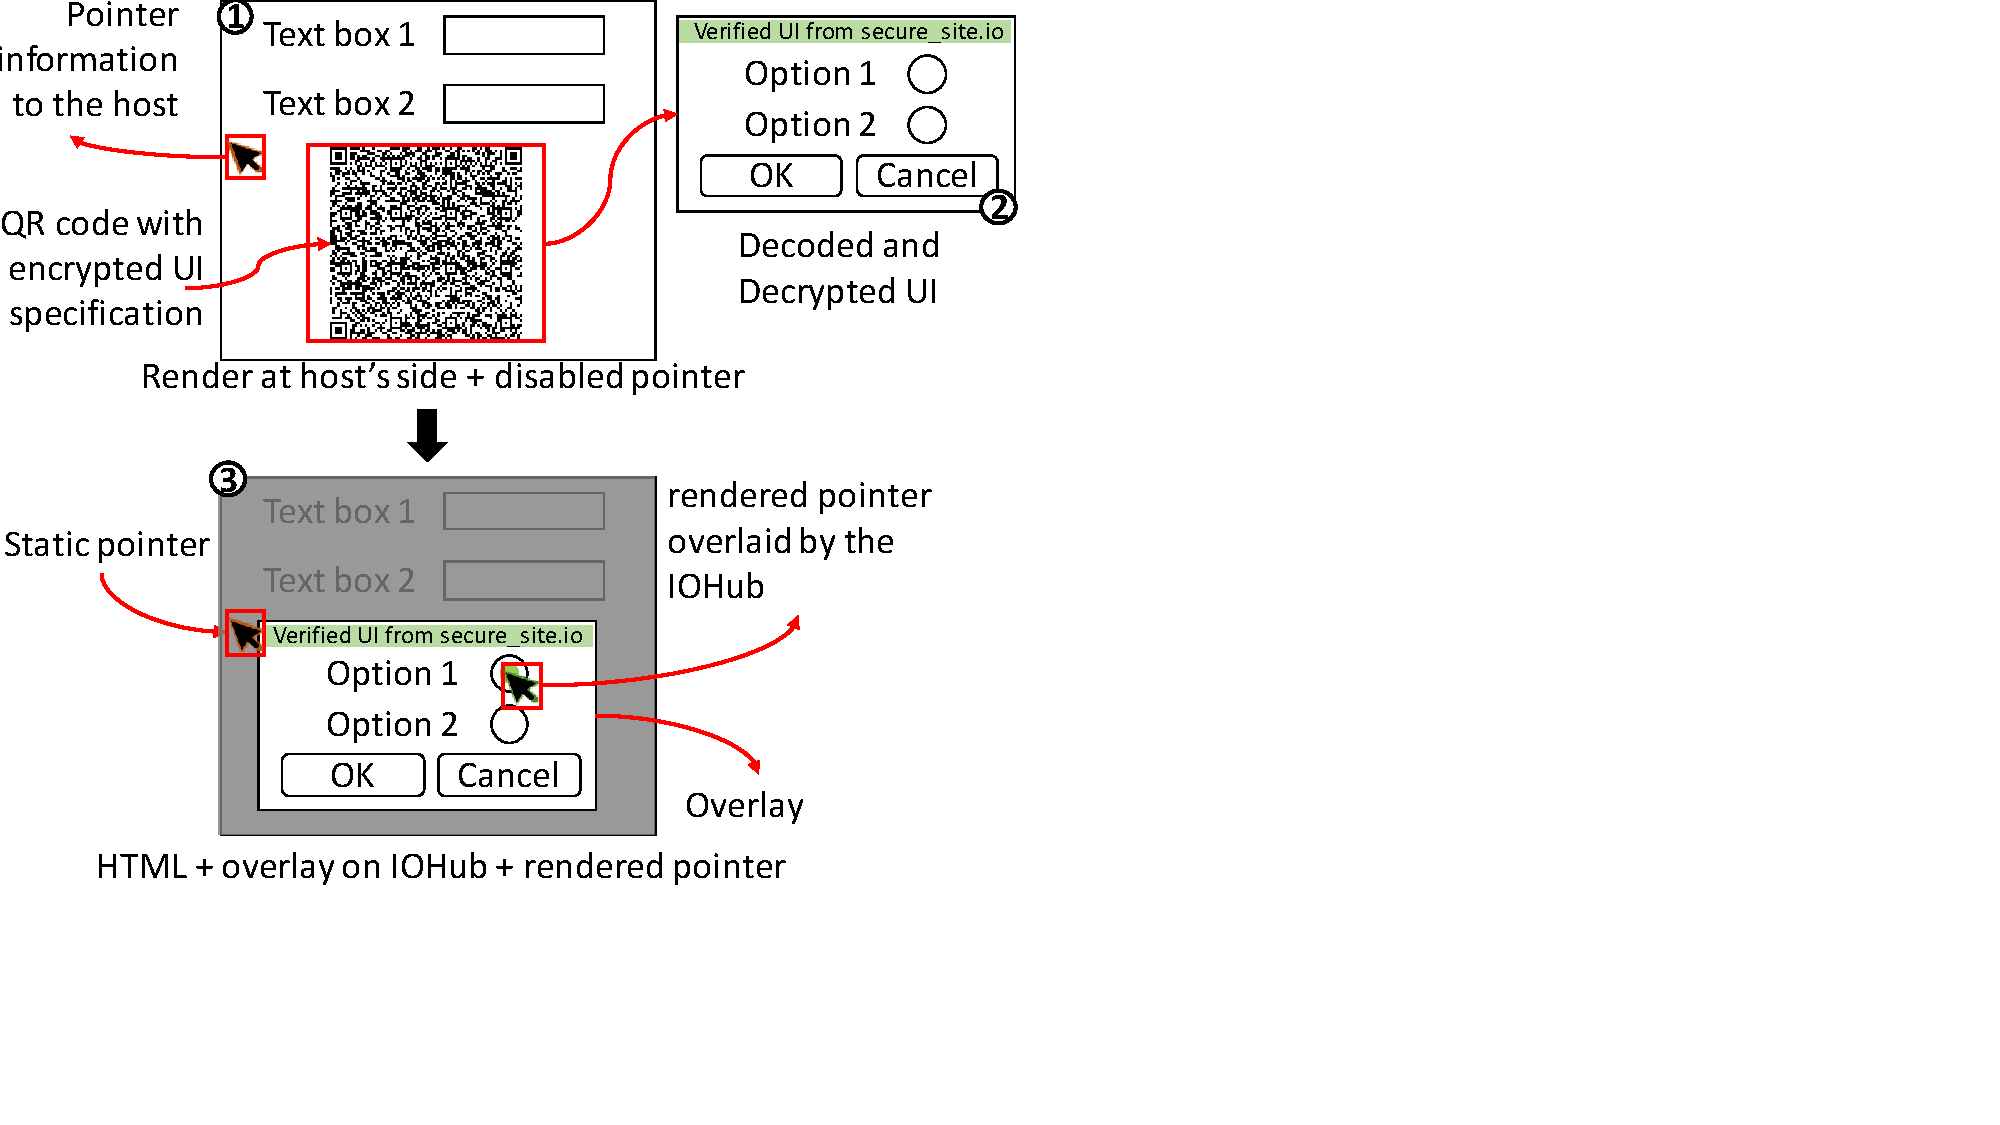
\includegraphics[trim={0 4cm 17cm 0}, clip, width=0.8\linewidth]{activityPrivacyRender.pdf}
\caption{\textbf{Activity privacy.}}
\label{fig:activityPrivacy}
\centering
\end{figure}


\subsection{Activity Privacy}
\label{sec:systemDesign:mousePrivacy}

The host system can be made fully oblivious of the mouse pointer, user activity and UI for a small portion of the browser that handles sensitive data or operations. We call this part of the display \emph{Oblivious Window} (OW). We opted out from the device rendering the HTML element inside the OW. Figure~\ref{fig:activityPrivacy} shows the overall construct of this idea. The server stores pre-rendered images corresponding to the OW and send the encrypted image along with the HTML page to the host system. The host renders the webpage along with an encrypted OW encoded as a QR code. The content of the QR code is encrypted with the \tls key that is shared between the device and the remote server.

The flow of the system can be divided into three parts: initialization, operation, and update.

\myparagraph{Initialization.} The initialization phase establishes a secure channel between the device and the remote server over the HTTP channel between the host and the remote host. The \js snippet that is served by the remote server handles the handshake between the device and remote server that is required to establish the secure channel. The flow of the system is the following: 
\begin{enumerate}
  \item The user initiates a new session by pressing a button on the device. This makes the device ready for an initialization phased with a remote server.
  \item When the user loads the web page from the remote server for the first time, the remote server sends its public certificate signed by a CA encoded in a QR code. 
  \item The device reads the QR and sends keyboard events that encode the signed public certificate of the device's public key in base64 encoded format. The \js served by the remote serve gets the keystrokes and generates a \texttt{XMLHttpRequest}.
  \item After exchanging the signed public certificates, the device and the remote server generates a shared secret that is used to encrypt and authenticate communications between the device and the remote server.
\end{enumerate}


\subsection{Output Privacy}
\label{sec:systemDesign:outputPrivacy}

\name provides output privacy and integrity protection of the output. One can think of this property as the ability to retrieve information from the remote server and display it to the user where the host system remains oblivious to the sensitive information. The overall flow of the system is illustrated in Figure~\ref{fig:outputPrivacy}. The steps are the following:

\begin{enumerate}
  \item[\one] The server sends the webpage and the encrypted data to the host over the \http connection between the browser and the remote server.
  \item[\two] The host generates the display frames and the encrypted data from the server and send them to the \device over the HDMI.
  \item[\three] The \device decrypts the encrypted data and overlay them on the frames that are received from the host.
  \item[\four] The \device sends the frames and corresponding overlays to the display device where the user sees them.
\end{enumerate}


\subsection{Side-channel Leakages frm the Activity Privacy}
\label{sec:systemDesign:sideChanneLeakage}







